\documentclass[11pt, a4paper]{article}
\usepackage[a4paper, total={6in, 8in}]{geometry}
\usepackage{graphicx}
\usepackage{float}
\graphicspath{{../img/}}
\renewcommand{\abstractname}{Overview}

\begin{document}
  \title{Pinyin Plotter: Visualizing the Tones of Mandarin Chinese}
  \author{Dustin Chung}
  \date{Project: May 2018 | Report: July 2018}
  \maketitle

  \begin{abstract}
    Spoken Mandarin Chinese has 5 tones: flat, rising, v-shaped, falling, and clear. The meaning of words can change depending on the tones used. The Pinyin notation uses romanized, accented words indicate how the syllables should be pronounced. In this project, the tone marker "accents" are interpreted literally as isolated graphs that are concatenated and plotted, forming a 2D "landscape". It was found that the 4th, "falling" tone is the most prevalent in most Chinese works. This is possibly due to the use of the 4th tone in commonly appearing grammar structures or words. In addition, it could be that the language was formed with a bias towards the 4th tone as it is the easiest to pronounce compared to the others.
  \end{abstract}

  \section{Introduction}
    The tones of Mandarin chinese are as follows:
      \begin{itemize}
        \item First, flat tone
        \item Second, rising tone
        \item Third, V tone
        \item Fourth, falling tone
        \item Fifth, neutral (clear) tone
      \end{itemize}

    In the Pinyin Plotter project, the accents above the vowels are interpreted literally as segments of linear graphs which are then concatenated to form one continuous line. Each accent and its respective isolated graphical equation is given below:

    \begin{itemize}
      \item First, flat tone: $y = 1 + c$
      \item Second, rising tone: $y = x + c$
      \item Third, V tone: $y = |2x| + c$ (steeper gradient accounts for the fact that the line must go down AND back up)
      \item Fourth, falling tone: $y = -x + c$
      \item Fifth, neutral (clear) tone: Not plotted
    \end{itemize}

  \section{Methods}
    The first step in processing the accents is to first convert the Chinese into Hanyu Pinyin. This is easily done online as there are plenty of converters. Once the pinyin is loaded into the Python script, the script extracts all of the accents in order of appearance in the source text.

    The script then iterates through each collected accent and plots the respective line onto a graph with matplotlib. Each plot is limited to a certain domain of $x$. Since the gradients $m$ and step sizes (how many units of $x$ per plotted tone) are defined by us, (see Introduction) and the starting point of the graph is also defined as the origin $(x_0, y_0) = (0, 0)$, calculating the coordinates of the next plot point is trivial. For a predefined step size, t:

    \begin{equation}
      m =\frac{y_2 - y_1}{x_2 - x_1}
    \end{equation}
    \begin{equation}
      x_2 = x_1 + t
    \end{equation}
    \begin{equation}
      y_2 = m(x_2 - x_1) + y_1
    \end{equation}

  \section{Results and Discussion}
    The initial target data for Pinyin Plotter was Chinese songs. Below are the graph results for three random songs from China and Taiwan:

    \begin{figure}[H]
      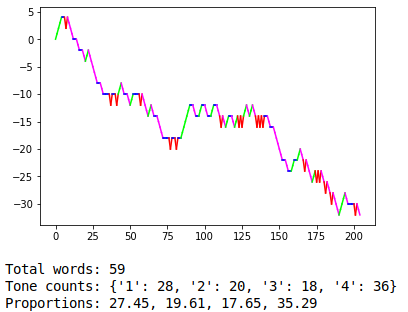
\includegraphics[width=8cm]{qnzl}
      \centering
      \caption{Plot of Chinese song 1}
    \end{figure}

    \begin{figure}[H]
      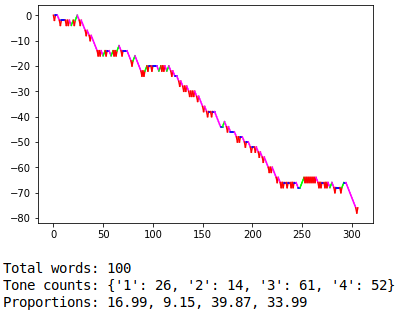
\includegraphics[width=8cm]{lsadm}
      \centering
      \caption{Plot of Chinese song 2}
    \end{figure}

    \begin{figure}[H]
      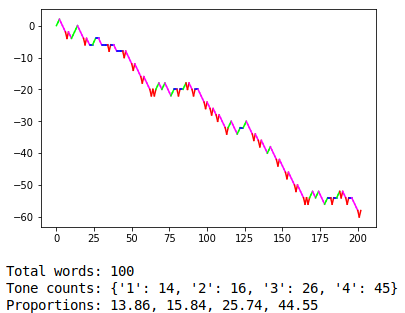
\includegraphics[width=8cm]{tmm}
      \centering
      \caption{Plot of Chinese song 3}
    \end{figure}

    It should be noted that typically, Chinese songs do not stress or even omit the tones, as singing with the tones is not convenient whilst trying to maintain a melody. Knowing this, a news story from a randomly selected Chinese news website and an exerpt of old Chinese literature were also graphed:

    \begin{figure}[H]
      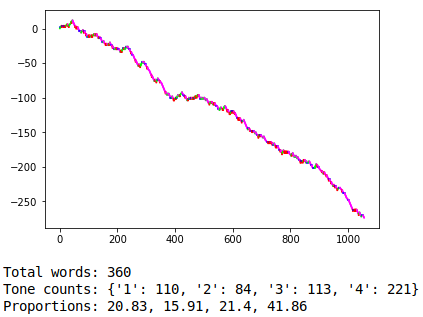
\includegraphics[width=8cm]{cn_news}
      \centering
      \caption{Plot of Chinese news story}
    \end{figure}

    \begin{figure}[H]
      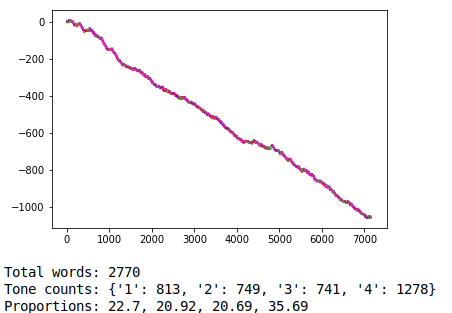
\includegraphics[width=8cm]{liafs}
      \centering
      \caption{Plot of Chinese literature exerpt}
    \end{figure}

    It can be seen that all the tested sources show a strong downward fall- indicating the dominance of the 4th falling tone. These results are in agreement to a similar undertaking performed and reported on Quora in 2012, that determined that the 4th tone was most prevalent.\cite{quora}

    The question remains: why are the falling tones more prevalent? The author can only guess that when the language was first being developed, the easiest tone for one to sound out would be the fast falling tone (as opposed to the other 3 tones, which are more drawn out).

    \section{Conclusions and Future Work}
      A Python script was made that parsed the tones of Hanyu Pinyin and used the shapes of the accents themselves to plot them on a graph. It has been shown by testing text sources across different contexts (songs, news and literature) that the 4th falling tone of Chinese is the most prevalent, with all graphs veering downwards- reflecting the downward sound of the 4th tone.

      As only 5 text sources were tested, future work could entail testing more sources of text in different contexts (e.g. non-fiction books, scientific journals).

      Work can also be done on the Python script itself: if the script could take the actual Chinese characters as input and convert them in to Pinyin automatically, it not only saves the step of having to do the conversion manually but also allows us to analyze the frequency of the Chinese characters. This improvement would allow one to see if certain characters are heavy contributors to a certain tone quantity, and maybe even find out why the 4th tone is so prevalent overall.

    \begin{thebibliography}{1}
      \bibitem{quora}
      Lin. K; Quora; https://tinyurl.com/y75nlfft; 2012
    \end{thebibliography}
\end{document}
